\documentclass[12pt]{report}

\usepackage[a4paper,
            left=2.5cm,
            right=2.5cm,
            top=2.5cm,
            bottom=2.5cm]{geometry}

\usepackage[english]{babel}
\usepackage{packages/sleek-title}
\usepackage{packages/sleek-listings}
\usepackage{setspace}
\usepackage{apacite}
\usepackage{multirow}
\usepackage{subcaption}

%%%%%%%%%%%%%%
% Title-page %
%%%%%%%%%%%%%%

\institute{University of Economics and Law}
\faculty{Faculty of Information Systems}
\logo{./resources/pdf/logo.pdf}

\title{FINAL REPORT}
\subtitle{Credit Card Approval Prediction: A comparative analysis between Logistic Regression, Causal Forest, XGBoost, and RandomForest}
\context{Course: Artificial Intelligence in Business Analytics}

\author{\textit{Students}\\Nguyen Thi Huong Giang\\Nguyen Thi Yen Kieu\\Le Minh Nguyen\\Dang Anh Nhu\\Le Huynh Thuy Vy}
\supervisor{\textit{Lecturer}\\Le Hoanh Su, PhD.\\Trinh Quang Viet, PhD.}

\date{December 2024}

\onehalfspacing

\begin{document}

    \maketitle

    \chapter*{Acknowledgements}
    First of all, we would like to express our sincere gratitude for your unwavering support and motivation throughout this project. Your enthusiasm and dedication as our project supervisor have been instrumental in our success. We are particularly grateful for the time you invested in teaching and guiding us from the project's inception to its completion.
    
    We would also like to extend our thanks for your invaluable advice and assistance during the project. The knowledge you imparted has proven to be both valuable and practical. We appreciate the favorable conditions you created for us to excel in our studies and project implementation.
    
    We acknowledge that, despite your guidance and the time constraints we faced, there may be shortcomings in our final project. However, we are confident that the skills and knowledge we gained under your supervision will be invaluable assets in our future endeavors.
    
    Finally, we would like to express our gratitude to our families for their unwavering support and encouragement throughout our studies.
    
    \begin{flushright}
        Group Casual
    \end{flushright}

    \chapter*{Commitment}
    We undertake that this report is completed based on the results of our research and that the results of this report have not been used for any other peer report.

    \begin{flushright}
        Ho Chi Minh City, 12/2024\\
        Group Casual
    \end{flushright}

    \begin{abstract}
        This report presents a comprehensive analysis of credit card approval prediction using various machine learning algorithms, including Logistic Regression, Random Forest, Causal Forest, and XGBoost. The study aims to evaluate the effectiveness of these models in improving the accuracy, efficiency, and fairness of the credit card approval process. The research involves extensive data preprocessing, feature engineering, and the application of causal inference techniques to identify key factors influencing credit card approval decisions. The results demonstrate that while traditional models like Logistic Regression and Random Forest perform well, the integration of causal AI provides significant improvements in transparency and predictive accuracy. The findings highlight the potential of advanced machine learning and causal inference methods in enhancing financial decision-making processes. Future work includes integrating macroeconomic indicators and user behavioral data to further refine the models and developing early warning systems for proactive risk management.
    \end{abstract}

    \tableofcontents
    \listoffigures
    \listoftables

    \chapter{Introduction}
    This chapter provides an overview of the research, including the research context, scope, methodology, and objectives.

    \section{Research Problem}
    The demand for credit cards has rapidly increased due to both the convenience of payments and the strong growth of online shopping, financial services, and consumer loans. This trend has significantly increased credit card applications, placing pressure on the traditional approval process, which often relies on fixed indicators like credit scores, income, and users' financial history. However, with an ever-growing and diverse dataset, relying solely on these factors risks overwhelming the approval process, leading to errors and inadequate accuracy and fairness.

    Nowadays, credit profiles can include complex data such as transaction history, spending trends, and even non-traditional factors like online activity or social media information. This additional data provides financial institutions with a multi-dimensional view of clients, particularly in assessing payment capabilities. However, integrating and analyzing such complex data requires advanced processes and technology that traditional methods cannot optimally meet.

    This study focuses on evaluating whether modern machine learning algorithms like Logistic Regression, RandomForest, Causal Forest, and XGBoost can help improve the accuracy, efficiency, and fairness of the credit card approval process. These algorithms not only enable automation but also can process and analyze large volumes of multi-dimensional data, uncovering complex relationships among credit factors. By applying these machine learning models, the research aims to offer a superior credit card approval prediction solution, reducing risks while ensuring fair assessments, thereby enhancing the quality and speed of financial institutions' processing.

    \section{Research Subjects}
    The study's subjects are credit card application profiles, including applicant demographic information, financial history, and employment details. This data provides a comprehensive view of applicants' creditworthiness, serving as the primary input for machine learning algorithms to make predictive decisions. By analyzing characteristics such as age, gender, total debt, annual income, and credit scores, the research can identify key factors influencing approval decisions.

    \section{Outline}

    The structure of the thesis study is outlined as follows:
    \begin{itemize}
        \item Chapter 1 provides an introduction to the topic, presenting the problem statement, objectives, and research questions to clarify the study’s purpose.
        \item Chapter 2 covers the research background, offering an introduction to the main topics relevant to the study.
        \item Chapter 3 reviews related work, examining prior research and relevant aspects that support the study’s focus.
        \item Chapter 4 outlines the methodology, detailing the selected methods, datasets, and procedural steps of the algorithm.
        \item Chapter 5 presents and analyzes the results, offering a comprehensive discussion of the findings based on the applied methods.
        \item Chapter 6 dives into an in-depth discussion of the results, including any potential validity concerns within the work.
        \item Chapter 7 concludes the thesis, summarizing key insights and suggesting potential directions for future research.
    \end{itemize}

    \section{Objective}
    This research aims to evaluate and select the most effective predictive model for the credit card approval process, helping financial institutions optimize the accuracy, fairness, and efficiency of approval decisions. The objectives include:

    {\bfseries Objective 1:} Identify the best machine learning model for predicting credit card approval by comparing Logistic Regression, Causal Forest, and XGBoost. The study will assess each model's effectiveness in classifying applicants according to creditworthiness conditions.

    {\bfseries Objective 2:} Improve fairness and transparency in the credit card approval process. The research focuses on model performance and factors such as accuracy in assessment and error reduction in approval decisions, ensuring fair, unbiased credit card approvals.

    {\bfseries Objective 3:} Develop an automated and fairer credit approval process that allows financial institutions to streamline credit assessment. The study aims to offer a widely applicable automation solution that meets the increasing demands of the financial industry.

    \chapter{Background}
    
    \section{Machine Learning}
    Machine Learning (ML) is a branch of Artificial Intelligence (AI) that enables systems to learn and adapt on their own. Rather than relying on explicit programming for each task, ML systems are designed to improve and evolve through experience. This means that they can autonomously analyze data, learn from it, and make adjustments without needing specific instructions for every scenario.

    \subsection{Supervised Learning}
    Supervised learning is a foundational method in machine learning, where machines learn similarly to how people improve through experience and feedback. By providing relevant data and setting criteria for evaluation, we guide the machine in learning to make accurate predictions. This guidance, or "supervision," involves showing the machine examples of correct and incorrect outcomes for a given task.

    In this approach, the machine uses mathematical methods to establish a mapping between input and output variables, which it can then apply to predict results on new, unseen data. The success of a supervised learning model relies on the accuracy of this mapping. When inaccuracies are detected, adjustments are made to refine the model and enhance its learning capabilities.

    Supervised learning is broadly applied across various fields and is typically categorized into two main types, depending on the output type expected:
    
    \begin{itemize}
        \item {\bfseries Classification:} This technique is used to assign categorical labels to new data points based on patterns found in past data. Classification models are designed to identify and label data instances into predefined categories, which is essential for tasks like spam detection, sentiment analysis, and disease diagnosis. Using datasets with input features paired with their respective class labels, classification algorithms learn relationships within the data to make precise predictions.
        \item {\bfseries Regression:} Unlike classification, regression focuses on predicting continuous numerical values rather than categories. The objective of regression is to model the relationship between input features and continuous target values, allowing for predictions on new data points. This is particularly useful for applications such as stock price forecasting, demand prediction, and temperature modeling, where numerical outcomes are required.
    \end{itemize}

    \subsection{Unsupervised Learning}
    Unsupervised algorithms play a crucial role in machine learning by processing unlabeled datasets, which lack specified output variables. The primary function of these algorithms is to reveal hidden patterns and structures in unstructured data, allowing businesses to gain valuable insights. Core applications include grouping similar data points (clustering) and reducing the complexity of data (dimensionality reduction). Through exploratory data analysis, unsupervised learning provides organizations with meaningful information to enhance decision-making and stimulate innovation.

    Unsupervised learning is commonly divided into two main categories:
    \begin{itemize}
        \item {\bfseries Clustering:} Clustering organizes data points into groups based on their similarity, helping to uncover patterns and relationships in data without needing labeled examples.
        \item {\bfseries Association:} Association rule learning identifies relationships between items within a dataset. This technique uncovers rules indicating the likelihood that the presence of one item implies the presence of another, supporting pattern discovery within data.
    \end{itemize}

    \subsection{Semi-supervised Learning}
    While supervised learning is often computationally intensive and suited to a limited range of applications, unsupervised learning has broader applicability yet may fall short in addressing certain types of problems. Semi-supervised learning offers a balanced approach by utilizing both labeled and unlabeled data, thereby overcoming some of the limitations of purely supervised or unsupervised methods. In this approach, there is typically a large amount of unlabeled data and a smaller set of labeled data. Unsupervised methods initially cluster the unlabeled data, and the labeled data is then applied to infer labels for the grouped unlabeled data, expanding the labeled dataset.
    
    Semi-supervised learning includes two subcategories:

    \begin{itemize}
        \item {\bfseries Pure semi-supervised:} This approach follows an open-world assumption, where the datasets are considered independently of specific test samples.
        
        \item {\bfseries Transductive learning:} This approach operates under a closed-world assumption, where datasets are treated as test samples, optimizing performance specifically for those datasets.
    \end{itemize}

    \section{Machine Learning Algorithms}
    This section presents an overview of the machine learning algorithms used in this project.

    {\bfseries Logistic Regression Classifier (LRC)}
    
    Logistic regression is a statistical method for predicting the probability of a binary outcome by examining the relationship between one or more independent variables and a dependent variable. In this project, logistic regression is applied to analyze factors such as income, credit history, and employment status to estimate the likelihood of credit card approval. This technique’s ability to transform complex interactions into a probability score between 0 and 1 provides a clear and quantifiable link between each factor and the approval decision. By incorporating logistic regression, we enhance the accuracy of predictions and foster a fairer, more efficient credit approval process. The model was selected for its straightforward interpretability and computational efficiency, making it an ideal choice for financial data where understanding the influence of individual variables on decision outcomes is essential.

    {\bfseries Random Forest Classifier (RFC)}
    
    The Random Forest Classifier builds multiple decision trees, each trained on a portion of the dataset, to contribute to the model's overall output. Once these trees are generated, their individual predictions are aggregated through majority voting, enhancing the model's accuracy and stability. By utilizing multiple trees, the Random Forest ensures that each tree's learning is based on a dataset with similar distribution patterns, helping to minimize biases. This approach effectively addresses class imbalance in datasets and is versatile, as it can handle both classification and regression tasks.

    {\bfseries eXtreme Gradient Boosting (XGBoost)}

    XGBoost is widely recognized for its ability to build decision trees sequentially, prioritizing both computational efficiency and model performance. This technique assigns weights to individual features, which are then applied in the construction of decision trees to enhance prediction accuracy. Each tree addresses residual errors from previous predictions, leading to progressively more accurate results as multiple models are combined.  In our analysis, we aim to demonstrate XGBoost's ability to manage data imperfections, a critical factor in establishing precise and equitable credit approval models in the financial sector.

    {\bfseries Causal Forest}

    Causal forests are a causal inference method derived from Random Forests. While Random Forests repeatedly split data to reduce the prediction error of an outcome variable, Causal Forests focus on maximizing the differences in the relationship between an outcome variable and a "treatment" variable across splits. This approach aims to reveal variations in treatment effects across the sample, allowing for a deeper understanding of how the impact of a treatment may differ among different groups within the data

    \section{Data Preprocessing}

    Data preprocessing is a vital step in preparing datasets for machine learning model training, as it ensures the quality and reliability of the data. For this project, the credit card approval dataset underwent a series of preprocessing techniques to make it ready for analysis and model development. Each preprocessing step was carefully designed to address specific challenges found in real-world financial data, including handling missing values, transforming categorical data, and managing class imbalance.

    {\bfseries Label Encoding:} Label encoding is used to convert categorical data into a numerical format, a requirement for most machine learning algorithms. This technique assigns a unique integer to each category, where the first unique category in the dataset is represented by 0, the next by 1, and so on, until all categories are numerically encoded. By transforming categorical data into numerical form, label encoding enables algorithms to effectively process and learn from these features, allowing categorical data to be seamlessly integrated into predictive modeling. This step is critical in ensuring that categorical information can be interpreted and utilized by the model during training and analysis.

    {\bfseries Data Normalization (Min-Max Scaling):} Min-Max Scaling, commonly known as data normalization, is a crucial preprocessing method that adjusts the range of numerical features within a dataset. Unlike Standard Scaling, which normalizes data to a mean of zero and a standard deviation of one, Min-Max Scaling transforms values to fall within a specified range, typically from 0 to 1. This transformation is done using the formula:

    \[X_{norm} = \frac{X - X_{min}}{X_{max} - X_{min}}\]

    Where X represents the original data point, and Xmin and Xmax are the minimum and maximum values of the feature, respectively. Min-Max Scaling is particularly effective when features have varying scales, as it standardizes these differences and allows algorithms to perform optimally by preventing any single feature from disproportionately influencing the model. Normalized data can help the model train more quickly and yield improved performance.

    {\bfseries Class Imbalance:} Class imbalance poses a significant challenge in machine learning, as models may become biased towards the majority class. To address this, techniques such as resampling, cost-sensitive learning, and adjustments to algorithm parameters can be applied. Instead of relying on traditional accuracy, performance is more accurately measured with precision, recall, and F1-score metrics, which offer a balanced view of the model’s effectiveness across classes. These methods ensure the model is fair and robust, making it suitable for real-world applications with imbalanced data.

    {\bfseries Train-Test Split:} Dividing the dataset into training and testing sets is essential for evaluating the model's performance on unseen data. The {\bfseries \texttt{train\_test\_split}} function from Python’s {\bfseries \texttt {sklearn.model\_selection}} library is commonly used to separate the dataset into these two sets, enabling accurate performance assessments and minimizing overfitting risks. In Python, this function is typically used as follows:

    \begin{lstlisting}[style=default, language=python*, gobble=3]
        train_test_split(X, y, train_size, test_size, random_state)
    \end{lstlisting}

    Here, X and y represent the feature matrix and target vector, respectively. The \texttt{test\_size} parameter defines the proportion of the dataset to be used for testing and can be a float (between 0.0 and 1.0) or an integer specifying the number of samples. Conversely, \texttt{train\_size} indicates the portion allocated to the training set. Setting \texttt{random\_state} ensures that data is consistently shuffled, allowing for reproducibility across different runs.

    \section{Classification Evaluation Metrics}

    {\bfseries Confusion Matrix}

    A confusion matrix is a tool used to evaluate the effectiveness of a classification model by comparing its predictions with the actual values of the target variable. This matrix is essential for calculating key metrics such as accuracy, precision, recall, and F1 score. It organizes the results of a binary classification task into four possible outcomes:

    \begin{itemize}
        \item {\bfseries True Positive (TP)}: The model correctly predicts a positive outcome, matching the actual positive label.
        \item {\bfseries False Positive (FP)}: The model incorrectly predicts a positive outcome, while the actual label is negative.
        \item {\bfseries True Negative (TN)}: The model correctly predicts a negative outcome, matching the actual negative label.
        \item {\bfseries False Negative (FN)}: The model incorrectly predicts a negative outcome, while the actual label is positive.
    \end{itemize}

    {\bfseries Accuracy}

    Accuracy measures the proportion of correct predictions made by the model out of the total predictions. While it offers a basic overview of model performance, accuracy alone may be misleading, especially when dealing with imbalanced datasets, as it may not reflect the model’s effectiveness in capturing minority class predictions.

    \[Accuracy = \frac{TP + TN}{TP + TN + FP + FN}\]

    {\bfseries Precision}

    Precision represents the ratio of true positives to the total number of instances predicted as positive. It measures the accuracy of positive predictions, which is particularly important when minimizing false positives is critical. The formula for precision is:

    \[Precision = \frac{TP}{TP + FP}\]

    {\bfseries Recall}

    Recall, or sensitivity, is the ratio of true positives to the total number of actual positive instances. This metric reflects how effectively the model identifies true positive cases, which is essential when the cost of false negatives is high. The formula for recall is:

    \[Recall = \frac{TP}{TP + FN}\]

    {\bfseries F1 Score}

    The F1 Score is the harmonic mean of precision and recall, providing a balanced evaluation of these two metrics. This score is particularly useful when both false positives and false negatives carry significant weight. The formula for the F1 Score is:

    \[F1\ Score = 2 \times \frac{Precision \times Recall}{Precision + Recall}\]

    \section{Working Environment}
    This experiment was conducted using Google Colab, a cloud-based computing platform. Google Colab provides substantial computing power without placing demands on the local system’s CPU and RAM, making it more efficient than most laptops. Various Python libraries were used in this thesis, including Pandas, Scikit-learn, Matplotlib, and NumPy.

    {\bfseries Pandas}

    Pandas is a widely-used open-source Python library designed for data cleaning, manipulation, and analysis. It supports data input from multiple sources, including CSV, Excel, SQL, and JSON files. Pandas offers two primary data structures: the one-dimensional Series and the two-dimensional DataFrame, making it versatile for handling and analyzing data. Version 1.3.5 of Pandas was used in this thesis.

    {\bfseries Scikit-learn}

    Scikit-learn, also known as sklearn, is a powerful open-source library for data analysis, preprocessing, and machine learning algorithms. Built on top of NumPy, SciPy, and Matplotlib, it emphasizes performance and scalability. The version of Scikit-learn used in this thesis was 1.0.2.
    
    {\bfseries Matplotlib}

    Matplotlib is an open-source library for scientific and technical computing in Python. It supports creating a variety of high-quality visualizations, including line plots, scatter plots, bar charts, and histograms. In this thesis, Matplotlib version 3.5.3 was employed.

    {\bfseries NumPy}

    NumPy, short for Numerical Python, is an open-source library that provides support for working with multidimensional arrays, matrices, and mathematical functions. It is especially useful for data analysis, preprocessing, and complex numerical operations. This thesis used NumPy version 1.21.6.

    {\bfseries DoWhy}

    DoWhy is a comprehensive library for causal analysis that integrates the latest advancements in modeling assumptions and robustness checks, providing a user-friendly API. Designed to guide users through best practices in causal inference, DoWhy’s API is structured around four fundamental steps: Model, Identify, Estimate, and Refute.
    \begin{itemize}
        \item {\bfseries Model:} Encodes prior knowledge into a formal causal graph.
        \item {\bfseries Identify:} Employs graph-based methods, like the ID algorithm, to recognize causal effects.
        \item {\bfseries Estimate:} Applies statistical methods, including sophisticated approaches from EconML, to evaluate the identified estimand.
        \item {\bfseries Refute:} Tests the validity of the causal assumptions and resulting estimates.
    \end{itemize}
    
    DoWhy combines two robust frameworks: causal graphs and potential outcomes. It leverages graph-based criteria and do-calculus to model assumptions and to identify non-parametric causal effects. For estimation, DoWhy incorporates methods based on potential outcomes, drawing on external libraries like EconML and CausalML. In 2022, DoWhy joined the community-governed PyWhy organization, a move aimed at fostering an open-source ecosystem for causal machine learning.

    {\bfseries EconML}

    EconML complements DoWhy by focusing on advanced estimation techniques grounded in the latest developments in causal machine learning. EconML applies state-of-the-art machine learning methods to estimate individualized causal effects from observational or experimental data, using supervised algorithms such as random forests, boosting, lasso, and neural networks to predict outcomes and improve on traditional methods through automated model selection with cross-fitting.

    Causal machine learning represents a major advancement by integrating machine learning within each stage of causal analysis. EconML provides a straightforward API, building on popular ML packages like scikit-learn, to make estimating causal effects accessible with minimal coding. Behind the scenes, EconML uses flexible ML models to estimate nuisance functions, with options like AutoML for algorithm selection, and applies cross-fitting to tune models, creating refined final models that deliver interpretable causal effects. Each estimation approach includes confidence intervals, many analytically constructed for efficiency, and supports modeling heterogeneous treatment effects to understand variation in treatment effects across a population, enabling tailored and personalized interventions.

    \chapter{Related Work}
    Several studies have examined machine learning algorithms for predicting credit card approval, exploring diverse methods and data conditions to improve prediction accuracy and model robustness. This section consolidates the relevant literature, specifically discussing algorithms central to this thesis: Logistic Regression, KNN, Decision Trees, Random Forest, and XGBoost.

    \citeA{Satchidananda2006Comparing} explored the effectiveness of Logistic Regression and Decision Trees in credit card approval systems, finding that while Logistic Regression provided a reliable baseline, Decision Trees performed better with non-linear data relationships, making them particularly effective for datasets with noise and variability.

    In a comparative study conducted in 2021, \citeauthor{Kibria2021Application}. evaluated deep learning, logistic regression, and support vector machines for predicting credit card approval. They assessed each model based on accuracy, precision, recall, and F1 score, concluding that the deep learning model achieved the highest accuracy at 87.10\%. This slightly exceeded the accuracy of logistic regression and support vector machines, which both attained 86.23\%, indicating a marginal advantage of deep learning in this context.

    \shortciteNP{Flores2022Classification} conducted an analysis of various machine learning classifiers on a credit card approval dataset, which was reduced to 12 attributes and 132,492 instances after data cleaning and feature selection. Using 10-fold cross-validation, they evaluated Random Forest (RF), K-Nearest Neighbors (KNN), and Neural Networks (NN) models based on metrics such as confusion matrices and ROC curves. Random Forest emerged as the top performer with an accuracy of 95.76\%, outperforming KNN (94.37\%) and Neural Networks (71.56\%), and achieved the highest scores across accuracy, precision, recall, specificity, and AUC.

    \shortciteNP{Lee2020Bootstrap} centered their research on Random Forest and XGBoost, examining their performance in noisy financial data. Their findings indicated that the robustness of Random Forest and the gradient boosting capabilities of XGBoost effectively mitigated the impact of Gaussian noise, resulting in enhanced predictive accuracy and model reliability.

    Building upon these insights, this thesis aims to investigate the effect of Gaussian noise on the predictive performance of these algorithms, as Gaussian noise is a frequent real-world challenge in credit card approval data. This study emphasizes the importance of evaluating each algorithm's capacity to handle noise, contributing to improved decision-making processes in credit approval systems.
    
    According to research by \shortciteNP{nandipati2024credit}, Logistic Regression, K-Nearest Neighbors (KNN), Decision Trees, Random Forest, and XGBoost models were applied to predict credit card approvals. The input data consisted of a credit card application dataset, supplemented with Gaussian noise to simulate real-world uncertainties. The models were trained through a process that included data normalization, handling class imbalance, and feature encoding, ensuring suitability for analysis. Results indicated that Random Forest and XGBoost demonstrated stronger noise resistance compared to other models, achieving accuracies of 53.7\% and 52.80\%, respectively, on both the unaltered and noise-added datasets. The study concluded that adding Gaussian noise enhances the robustness of predictive models under variable data conditions, with Random Forest and XGBoost identified as the most effective models in this context.

    \shortciteA{Carbo-Valverde2020Machine} applied the Causal Forest algorithm to study the digitization process among banking customers. Data was gathered from the Consumer Finance Survey, allowing for the identification of factors affecting the adoption and use of digital banking services. Causal Forest was used to estimate causal relationships and determine consumer decision sequences. The study's results revealed that checking account balances online had the largest impact on decisions to use online banking services, and that perceptions of service security were the most important factor influencing credit card usage. The study provides valuable recommendations for the banking sector in designing digitization strategies, emphasizing the need to create services that align with customer needs.

    According to \citeA{Lecca2021Machine}, machine learning algorithms such as Causal Forest have been applied to causal inference in biological networks. The study highlights that most current machine learning models primarily focus on correlation-based prediction rather than causation, posing limitations for applications in complex biological systems. By using the Causal Forest algorithm, the study successfully identified causal relationships among factors within biological networks, shedding light on how systems respond to external stimuli. The study underscores the potential of causal learning models to improve biological and medical analysis, which could lead to the development of better medical treatments.

    \shortciteA{Cheng2022Evaluation} conducted a study on evaluation methods for causal learning algorithms in the context of big data analytics. The research focused on evaluating the effectiveness of algorithms like Causal Forest using criteria such as Mean Squared Error (MSE), Precision, and Recall. A significant challenge noted was the lack of public benchmark data to support consistent evaluation. The study highlights the need for consistent and transparent evaluation standards to drive the practical advancement of causal learning models. The findings suggest that causal learning models hold great potential for enhancing decision-making capabilities, particularly in credit scoring and finance

    \chapter{Method}

    \begin{figure}[h]
        \centering
        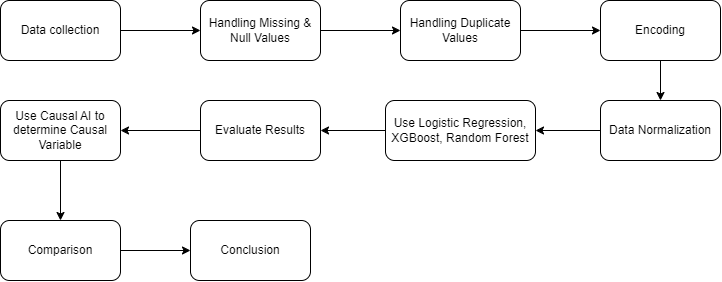
\includegraphics[width=0.8\textwidth]{resources/pic/Experimentation procedure.png}
        \caption{Experimentation procedure}
        \label{fig:Experimentation procedure}
    \end{figure}

    {\bfseries Data Collection:} Data was collected from reliable sources such as Kaggle, ensuring high-quality datasets. The data includes demographic information, credit history, and financial details of customers, enabling accurate prediction of credit card approvals.

    {\bfseries Handling Missing and Null Values:} Missing or null values were identified and addressed to ensure data integrity. For example, missing values in the "\texttt{OCCUPATION\_TYPE}" column were replaced with "Other" to retain the completeness of the dataset.

    {\bfseries Handling Duplicate Values:} Duplicate entries were detected in the "ID" column and removed, retaining only the first occurrence to avoid redundancy and ensure data accuracy.

    {\bfseries Data Encoding:} Categorical data was converted into numerical formats using label encoding to make it compatible with machine learning algorithms. For instance, the "Gender" column was encoded with 0 for female and 1 for male.

    {\bfseries Data Normalization:} Min-Max Scaling was applied to normalize numerical features, ensuring that all values fall within a range of 0 to 1. This step improves algorithm efficiency and prevents dominance of certain features in the learning process.
    
    {\bfseries Machine Learning Model Application:} Predictive models such as Logistic Regression, XGBoost, and Random Forest were developed to determine credit card approval probabilities. Hyperparameter tuning was performed to optimize each model’s performance, and the dataset was split into training (80\%) and testing (20\%) sets for evaluation.

    {\bfseries Model Evaluation:} Metrics such as accuracy, precision, recall, and F1-Score were calculated to assess model performance. Confusion matrices were analyzed to evaluate the accuracy of predictions for each target class.

    {\bfseries Causal Variable Identification Using Causal AI:} Causal AI was employed to identify variables with the strongest causal influence on the target variable. A causal graph was constructed to visualize relationships between input features and their effects on the outcome.

    {\bfseries Comparison of Results:} The performance of the models (Linear Regression, XGBoost, and Random Forest) was compared to identify the most effective solution. Additionally, results were benchmarked against previous studies to highlight improvements and adaptations.

    {\bfseries Conclusion and Insights:} Key findings and lessons learned from the research process were summarized. The effectiveness of Causal AI in enhancing accuracy and transparency was highlighted, alongside challenges encountered in applying causal methods in financial models. Recommendations for future research include integrating macroeconomic factors and behavioral data to improve accuracy and interpretability, as well as developing early warning systems for financial institutions.

    \section{Data Collection}
    \subsection{Dataset "Application Record"}
    \begin{itemize}
        \item {\bfseries Overview:} This dataset records detailed information about loan applications from customers at a financial institution. Each row represents a specific customer and includes demographic, financial, and personal information such as gender, marital status, education level, and occupation. This dataset helps highlight potential factors that influence credit approval and management decisions.
        \item {\bfseries Purpose:} The main goal of this dataset is to provide comprehensive information about customers when they apply for loans, enabling the institution to make informed credit decisions. It can be used to analyze personal characteristics that affect a customer's reliability in payment and to predict credit risk based on demographic and financial factors.
        \item {\bfseries Columns in the dataset:}
        \begin{itemize}
            \item {\bfseries \texttt{ID:}} Unique identifier for each customer.
            \item {\bfseries \texttt{CODE\_GENDER:}} Customer’s gender.
            \item {\bfseries \texttt{FLAG\_OWN\_CAR:}} Indicates whether the customer owns a car.
            \item {\bfseries \texttt{FLAG\_OWN\_REALTY:}} Indicates whether the customer owns real estate.
            \item {\bfseries \texttt{CNT\_CHILDREN:}} Number of children the customer has.
            \item {\bfseries \texttt{AMT\_INCOME\_TOTAL:}} Total annual income of the customer.
            \item {\bfseries \texttt{NAME\_INCOME\_TYPE:}} Type of income (e.g., salary, self-employed, retired).
            \item {\bfseries \texttt{NAME\_EDUCATION\_TYPE:}} Education level of the customer.
            \item {\bfseries \texttt{NAME\_FAMILY\_STATUS:}} Marital status of the customer.
            \item {\bfseries \texttt{NAME\_HOUSING\_TYPE:}} Type of housing the customer lives in.
            \item {\bfseries \texttt{DAYS\_BIRTH:}} Number of days since the customer was born (negative value represents age).
            \item {\bfseries \texttt{DAYS\_EMPLOYED:}} Number of days since the customer started employment.
            \item {\bfseries \texttt{FLAG\_MOBIL:}} Indicates if the customer has a mobile phone.
            \item {\bfseries \texttt{FLAG\_WORK\_PHONE:}} Indicates if the customer has a work phone.
            \item {\bfseries \texttt{FLAG\_PHONE:}} Indicates if the customer has a home phone.
            \item {\bfseries \texttt{FLAG\_EMAIL:}} Indicates if the customer has an email.
            \item {\bfseries \texttt{OCCUPATION\_TYPE:}} Occupation of the customer.
            \item {\bfseries \texttt{CNT\_FAM\_MEMBERS:}} Number of family members in the customer’s household.
        \end{itemize}
    \end{itemize}

    \subsection{Dataset "Credit Record"}
    \begin{itemize}
        \item {\bfseries Overview:} This dataset provides detailed information about each customer’s credit history, recorded monthly. Each row represents a monthly credit record for a customer, capturing payment status, including on-time payments, late payments, and account cancellations. These records are crucial for evaluating credit history and identifying potential signs of credit risk.
        \item {\bfseries Purpose:} The purpose of this dataset is to monitor and evaluate customers’ credit payment behavior over time. Tracking payment history enables the financial institution to identify customers with higher default risks, allowing for proactive risk management. Analyzing credit history helps to predict a customer’s future payment reliability based on past credit statuses.
        \item {\bfseries Key columns in the dataset:}
        \begin{itemize}
            \item {\bfseries \texttt{ID:}} Unique identifier for each customer, matching the "Application Record" dataset.
            \item {\bfseries \texttt{MONTHS\_BALANCE:}} Number of months since the current credit record (negative value indicates past).
            \item {\bfseries \texttt{STATUS:}} Customer’s payment status in that month, with codes as follows:
            \begin{itemize}
                \item 0: Paid on time.
                \item 1-5: Late payment with various levels.
                \item C: Credit account was canceled.
                \item X: No payment information for that month.
            \end{itemize}
        \end{itemize}
    \end{itemize}

    These two datasets are used together to analyze and evaluate customer debt repayment ability. By combining demographic factors (from the "Application Record") and credit history (from the "Credit Record"), financial institutions can build predictive models for credit risk. This information will enhance decision-making, minimize risk, and optimize credit management, leading to greater security in loan approval and debt recovery.

    \section{Data Pre-processing}
    Display the first 5 rows of the 'Application Record' dataset. These columns provide basic information related to the demographics and financial status of each individual in the dataset.
    
    \begin{lstlisting}[style=default, language=python*, gobble=3]
        df.head(5)
    \end{lstlisting}

    \begin{figure}[h!]
        \centering
        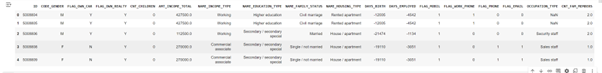
\includegraphics[width=0.8\textwidth]{resources/pic/Display the first 5 rows of the 'Application Record' dataset.png}
        \caption{Display the first 5 rows of the 'Application Record' dataset}
        \label{fig:Display the first 5 rows of the 'Application Record' dataset}
    \end{figure}

    Display the first 5 rows of the 'Credit Record' dataset. These columns provide detailed information about each customer's credit history, including payment status and account activity.

    \begin{figure}[h!]
        \centering
        \begin{tabular}{|c|c|c|c|}
            \textbf{ } & \textbf{\texttt{ID}} & \textbf{\texttt{MONTHS\_BALANCE}} & \textbf{\texttt{STATUS}} \\
            0 & 5001711 & 0.0 & X \\
            1 & 5001711 & -1.0 & 0 \\
            2 & 5001711 & -2.0 & 0 \\
            3 & 5001711 & -3.0 & 0 \\
            4 & 5001712 & 0.0 & C \\
        \end{tabular}
        \caption{Display the first 5 rows of the 'Application Record' dataset}
    \end{figure}

    Continue to check the number of rows and columns in each dataset. The results show that the 'Application Record' dataset has 438,557 rows and 18 columns; the 'Credit Record' dataset has 644,006 rows and 3 columns

    \begin{lstlisting}[style=default, language=python*, gobble=3]
        df.shape
        > (438557, 18)
        df2.shape
        > (644006, 3)
    \end{lstlisting}

    Next, descriptive statistics for columns with data type object (string or categorical) in the “Application Record” dataset.

    \begin{lstlisting}[style=default, language=python*, gobble=3]
        df.describe(include='object').T
    \end{lstlisting}

    \begin{figure}[h!]
        \centering
        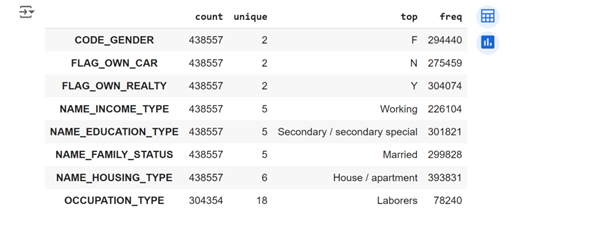
\includegraphics[width=0.7\textwidth]{resources/pic/Summary Statistics of Categorical Features in Dataset.png}
        \caption{Summary Statistics of Categorical Features in Dataset}
        \label{fig:Summary Statistics of Categorical Features in Dataset}
    \end{figure}

    Then use the info() function to provide an overview of the structure of the “Application Record” dataset which includes:
    
    {\bfseries Handle duplicate values.}
    
    Next, process the duplicate values in the “ID” column. The result shows that there are 47 duplicate values in the “ID” column.
    
    Check the number of duplicate ID values in the DataFrame.

    \begin{lstlisting}[style=default, language=python*, gobble=3]
        df['ID'].duplicate().sum()
        > 47
    \end{lstlisting}

    Delete rows with duplicate ID values, keeping only the first appearing ID value (first row). And check the results of duplicate ID values after deletion:

    \begin{lstlisting}[style=default, language=python*, gobble=3]
        df.drop_duplicates(subset='ID', keep='first')
        df['ID'].duplicate().sum()
        > 0
    \end{lstlisting}

    {\bfseries Finding the Cardinality in the data}

    Cardinality refers to the distinctiveness or uniqueness of values in a dataset or database column. It represent the number of unique values in a column or a set of column

    \begin{figure}[h!]
        \centering
        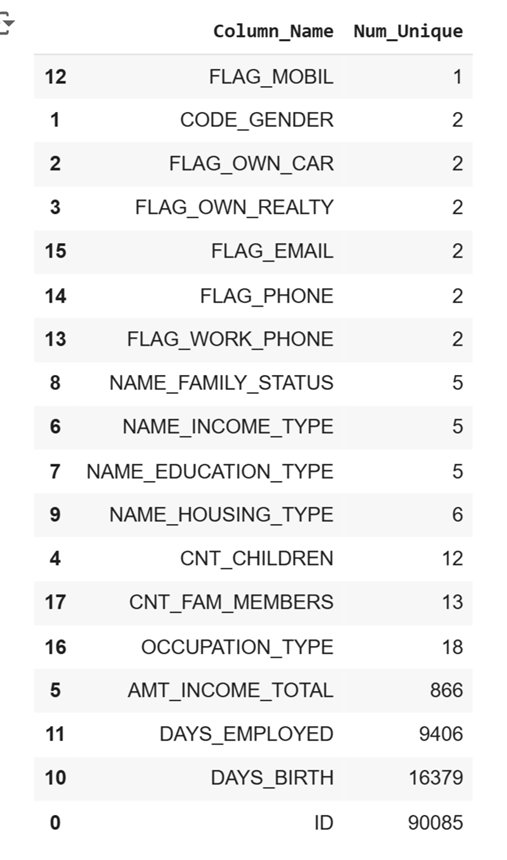
\includegraphics[width=0.4\textwidth]{resources/pic/Unique Value Count of Dataset Columns.png}
        \caption{Unique Value Count of Dataset Columns}
        \label{Unique Value Count of Dataset Columns}
    \end{figure}

    The observation reveals that the \texttt{FLAG\_MOBIL} column contains only a single unique value throughout the dataset. This indicates that the data in this column lacks variability, meaning that its value remains the same across all customers. As a result, this variable holds minimal significance in distinguishing between records, and it may be beneficial to exclude it from further analysis due to its limited contribution.

    \begin{lstlisting}[style=default, language=python*, gobble=3]
        df.drop(['FLAG_MOBIL'], axis=1, inplace=True)
    \end{lstlisting}

    {\bfseries Handling Missing Values}

    Handling missing values is crucial in data analysis, as they can compromise data quality and impact the accuracy and reliability of analytical or modeling outcomes. Properly addressing missing values helps prevent biased or partial insights, ensuring a more robust and valid analysis.

    \begin{figure}[h!]
        \centering
        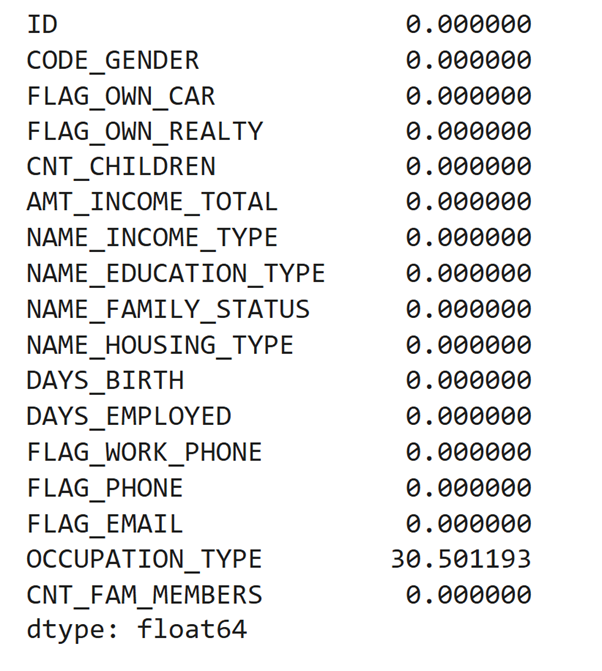
\includegraphics[width=0.4\textwidth]{resources/pic/Percentage of Missing Values in Dataset Columns.png}
        \caption{Percentage of Missing Values in Dataset Columns}
        \label{Percentage of Missing Values in Dataset Columns}
    \end{figure}

    It is evident that \texttt{OCCUPATION\_TYPE} stands out as the only column in the applications data with a significant amount of missing values. Managing these missing entries effectively is essential to maintain the integrity and accuracy of data analysis and modeling outcomes.
    
    To handle the missing values in \texttt{OCCUPATION\_TYPE} without removing rows, we opted to fill them with the value "Other." This approach ensures that the integrity of the dataset is maintained while accounting for missing information

    \begin{lstlisting}[style=default, language=python*, gobble=3]
        df['OCCUPATION_TYPE'].fillna('Other', inplace=True)
    \end{lstlisting}

    After rechecking for null values, it was confirmed that all columns now contain data, with no missing values remaining. This indicates that the previous handling of missing data was successful, resulting in a complete dataset ready for further analysis.

    \begin{figure}[h!]
        \centering
        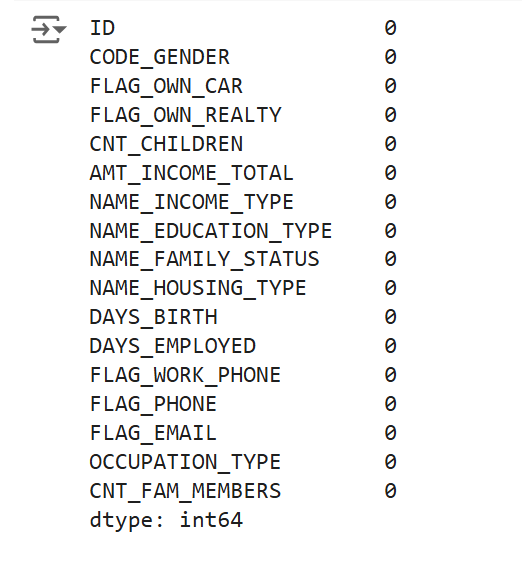
\includegraphics[width=0.4\textwidth]{resources/pic/Count of Missing Values in Dataset Columns after fill missing values.png}
        \caption{Count of Missing Values in Dataset Columns after fill missing values}
        \label{Count of Missing Values in Dataset Columns after fill missing values}
    \end{figure}

    \section{Exploratory Data Analysis}
    {\bfseries Converting data in proper format}

    In the “Credit Record” dataset, we transform \texttt{STATUS} data into a binary "target" variable to identify high-risk users, defined as those late on payments by 30 days or more. The result is a simplified indicator where \texttt{1} represents high-risk users and \texttt{0} represents low-risk, making the data ready for risk prediction or classification analysis.

    \begin{figure}[h!]
        \centering
        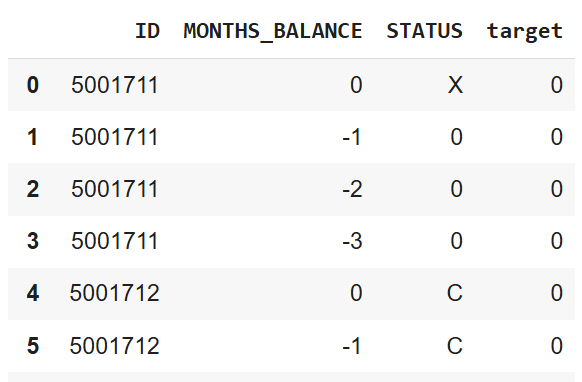
\includegraphics[width=0.7\textwidth]{resources/pic/Customer Credit Record with Target Variable.png}
        \caption{Customer Credit Record with Target Variable}
        \label{Customer Credit Record with Target Variable}
    \end{figure}

    Then, We combine two datasets based on the primary key ID.

    \begin{lstlisting}[style=default, language=python*, gobble=3]
        new_df = pd.merge(data, df, on=['ID'], how='inner')
    \end{lstlisting}

    The data is presented as shown below, providing an overview of its structure and content.

    \begin{figure}[h!]
        \centering
        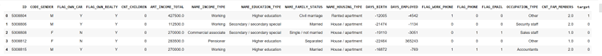
\includegraphics[width=\textwidth]{resources/pic/Overview of 2 datasets after combine.png}
        \caption{Overview of 2 datasets after combine}
        \label{Overview of 2 datasets after combine}
    \end{figure}

    {\bfseries Converting \texttt{DAYS\_BIRTH} Column to Readable Age Format}

    The \texttt{DAYS\_BIRTH} column provides information about an individual's age, but it's currently not in a readable format. We will convert it into a more understandable format to improve clarity.

    \begin{lstlisting}[style=default, language=python*, gobble=3]
        data['DAY_BIRTH']
    \end{lstlisting}

    \begin{figure}[h!]
        \centering
        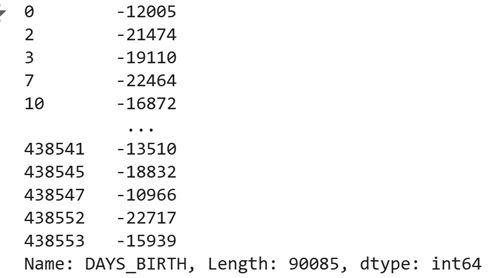
\includegraphics[width=0.8\textwidth]{resources/pic/‘DAYS BIRTH’ column.png}
        \caption{\texttt{DAYS\_BIRTH} column}
        \label{DAYS BIRTH column}
    \end{figure}

    The conversion uses the average length of a tropical year (365.2425 days) to achieve accurate age calculations.

    \begin{lstlisting}[style=numbered, language=python*, gobble=3]
        # Create age feature
        new_df['AGE_YEARS']=round(new_df['DAYS_BIRTH']/365.2425)
        # The number 365.2425 represents the average length of a tropical year
        # which is the time it takes for the Earth to complete a full orbit around the Sun.
        
        new_df['AGE_YEARS'].head()
    \end{lstlisting}

    \begin{lstlisting}[style=default, language=python*, gobble=3]
        > 0  33.0
        > 1  59.0
        > 2  52.0
        > 3  62.0
        > 4  46.0
        > Name: AGE_YEARS, dtype: float64
    \end{lstlisting}

    As now we have converted the \texttt{DAYS\_BIRTH} column into a proper format and named it as \texttt{AGE\_YEARS}. So now both are somewhat sharing same set of information in the data. So we will drop out the \texttt{DAYS\_BIRTH} for betterment of the data.

    {\bfseries Creating a Binary Indicator for Unemployment and Employment Status}

    We will create a binary unemployment indicator where \texttt{1} signifies unemployment and \texttt{0} signifies employment based on the \texttt{DAYS\_EMPLOYED} values in the dataset.

    \begin{figure}[h!]
        \centering
        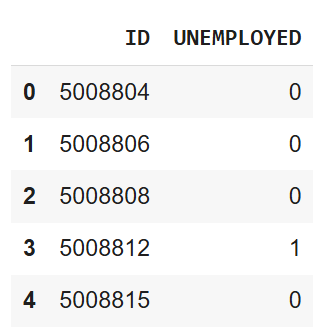
\includegraphics[width=0.65\textwidth]{resources/pic/‘ID’ and ‘UNEMPLOYED’ columns.png}
        \caption{\texttt{ID} and \texttt{UNEMPLOYED} columns}
        \label{ID and UNEMPLOYED columns}
    \end{figure}

    As now we have converted \texttt{DAYS\_EMPLOYED} column into a proper format and named it as \texttt{YEARS\_EMPLOYED}. So now both are somewhat sharing same set of information in the data. So we will drop out the \texttt{DAYS\_EMPLOYED} for betterment of the data.

    \begin{figure}[h!]
        \centering
        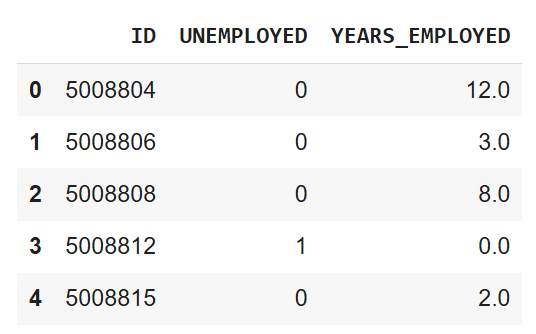
\includegraphics[width=0.75\textwidth]{resources/pic/‘ID’, ‘UNEMPLOYED’ and ‘YEARS_EMPLOYED’ columns.png}
        \caption{\texttt{ID}, \texttt{UNEMPLOYED} and \texttt{YEARS\_EMPLOYED} columns}
        \label{ID, UNEMPLOYED and YEARS EMPLOYED columns}
    \end{figure}

    {\bfseries Encode Binary Features}

    Below is a summary table of the binary encoding values applied to various categorical features, converting them into \texttt{0} and \texttt{1} for simplified processing in machine learning models:

    \begin{table}[h!]
        \centering
        \caption{Binary Encoding of Categorical Features}
        \begin{tabular}{|c|c|c|}
            \hline
            \textbf{Column} & \textbf{Original Category} & \textbf{Encoded Value} \\ \hline
            \multirow{2}{*}{\texttt{Gender}} & "F" (Female) & 0 \\
            & "M" (Male) & 1 \\ \hline
            \multirow{2}{*}{\texttt{Own\_car}} & "Y" (Yes, owns a car) & 1 \\
            & "N" (No, does not own a car) & 0 \\ \hline
            \multirow{2}{*}{\texttt{Own\_property}} & "Y" (Yes, owns property) & 1 \\
            & "N" (No, does not own property) & 0 \\ \hline
            \multirow{2}{*}{\texttt{Is\_Working}} & "Working", "Commercial associate", "State servant" & 1 \\
            & "Pensioner", "Student" & 0 \\ \hline
            \multirow{2}{*}{\texttt{Marital\_Status}} & "Civil marriage", "Married" & 1 \\
            & "Single / not married", "Separated", "Widow" & 0 \\ \hline
        \end{tabular}
    \end{table}

    Here is the dataset after data normalization, where categorical values have been encoded and the data has been transformed into a structured format suitable for machine learning models

    \begin{figure}[h!]
        \centering
        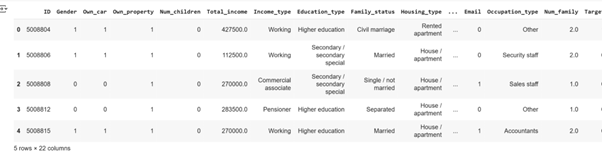
\includegraphics[width=0.8\textwidth]{resources/pic/dataset after data normalization.png}
        \caption{dataset after data normalization}
        \label{dataset after data normalization}
    \end{figure}

    {\bfseries Calculate the total size of each household}

    Calculates the total size of each household by adding the number of children to the number of adults (assumed based on marital status). This new \texttt{Household\_Size} feature could be useful for analysis or modeling, especially in scenarios where household composition is relevant.

    \begin{lstlisting}[style=default, language=python*, gobble=3]
        new_df['Household_Size'] = new_df['Num_children'] + new_df['Marital_Status'].apply(lambda x: 2 if x == 1 else 1)

              ID        Household_Size
        > 0   5008804   2
        > 1   5008806   2
        > 2   5008808   2
        > 3   5008812   1
        > 4   5008815   2
    \end{lstlisting}

    {\bfseries Dropping Unnecessary Columns}

    The goal of this process is to remove columns from the dataset that are not relevant to the analysis or machine learning models. In this case, the columns \texttt{ID}, \texttt{Email}, \texttt{Phone}, \texttt{Work\_phone}, \texttt{Num\_children}, \texttt{Is\_Working}, \texttt{Family\_status}, \texttt{Num\_family} are dropped from data as they likely contain personal identifiers or information that does not contribute to predictive features in the dataset. By removing these columns, we reduce the data's dimensionality and improve processing efficiency.

    {\bfseries Dataset for Model Training}

    These are the columns in the dataset prepared for modeling:

    \begin{figure}[h!]
        \centering
        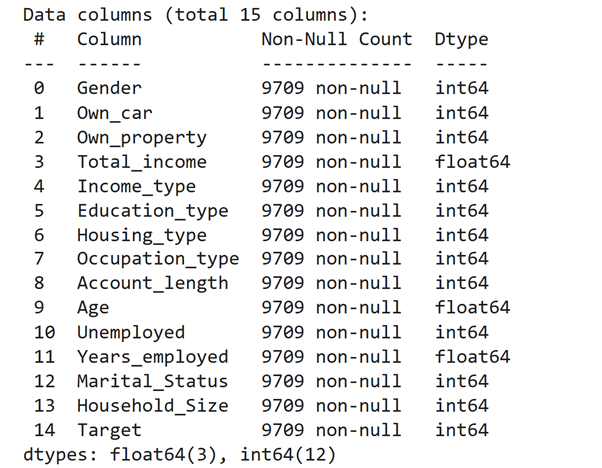
\includegraphics[width=0.5\textwidth]{resources/pic/dataset prepared for modeling.png}
        \caption{Dataset prepared for modeling}
        \label{dataset prepared for modeling}
    \end{figure}

    {\bfseries Data Visualization}

    \begin{figure}[h!]
        \centering
        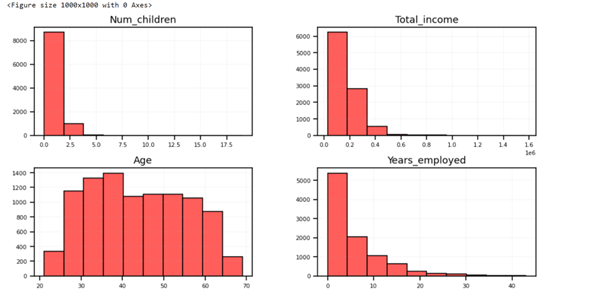
\includegraphics[width=0.8\textwidth]{resources/pic/Demographic and Employment Data Distribution.png}
        \caption{Demographic and Employment Data Distribution}
        \label{Demographic and Employment Data Distribution}
    \end{figure}

    The image figure displays histograms for four variables: Number of Children (\texttt{Num\_children}), Total Income (\texttt{Total\_income}), Age, and Years Employed (\texttt{Years\_employed}).

    \begin{itemize}
        \item The histogram for the number of children shows that most individuals have few or no children, with very few people having many children. This suggests a trend toward smaller family sizes, possibly influenced by financial pressures or a focus on career and personal development.
        \item The income distribution reveals a significant disparity, with the majority of individuals earning below 200,000 and only a small percentage earning high incomes. This indicates income inequality that may result from differences in job positions, education levels, or work experience.
        \item The age distribution indicates that most of the population falls within the 30 to 50 age range, which is considered the prime working age. This suggests that this group is likely in their career development phase, contributing significantly to the workforce.
        \item The distribution of years employed shows that most individuals have relatively few years of work experience, with the number of people with longer employment durations decreasing sharply. This pattern possibly indicates an influx of younger workers into the job market, with fewer people having extended work experience.
    \end{itemize}

    These histograms collectively reveal general demographic and employment trends within the population. The low number of children, high income disparity, and concentration of the workforce in middle working ages highlight a society focused on career and income, with notable income inequality. This trend could have implications for financial and social welfare policies, particularly those aimed at supporting low-income families or promoting work-life balance.

    \begin{figure}[h!]
        \centering
        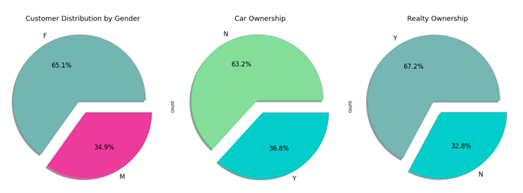
\includegraphics[width=0.8\textwidth]{resources/pic/Customer Demographics and Asset Ownership.png}
        \caption{Customer Demographics and Asset Ownership}
        \label{Customer Demographics and Asset Ownership}
    \end{figure}

    The figure displays three pie charts depicting the distribution of customers by gender, car ownership, and real estate ownership.

    \begin{itemize}
        \item The Gender Distribution pie chart shows that 65.1\% of customers are female (F), while 34.9\% are male (M). This indicates a higher representation of female customers in the dataset.
        \item The Car Ownership chart reveals that 63.2\% of customers do not own a car (N), whereas 36.8\% own a car (Y). This suggests that car ownership is less common among customers.
        \item The Real Estate Ownership chart indicates that 67.2\% of customers own real estate (Y), while 32.8\% do not (N). This implies that real estate ownership is more prevalent within the customer base compared to car ownership.
    \end{itemize}

    These charts provide an overview of customer demographics and asset ownership, highlighting a predominantly female customer base, lower car ownership, and relatively higher real estate ownership.

    \begin{figure}[h!]
        \centering
        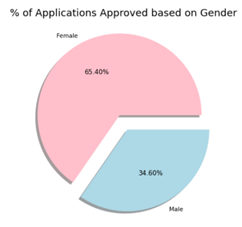
\includegraphics[width=0.8\textwidth]{resources/pic/Percent of Applications Approved Based on Gender.png}
        \caption{Percent of Applications Approved Based on Gender}
        \label{Percent of Applications Approved Based on Gender}
    \end{figure}

    The figure shows a pie chart representing the gender distribution of approved applications.

    The chart reveals that 65.4\% of the approved applications were from female applicants, while 34.6\% were from male applicants. This distribution suggests a higher approval rate among female applicants compared to male applicants within this dataset.

    The chart is color-coded with pink for female and light blue for male, making it easy to distinguish between the two groups visually. The gender-based approval disparity could imply underlying factors influencing application success rates between genders.

    \begin{figure}[h!]
        \centering
        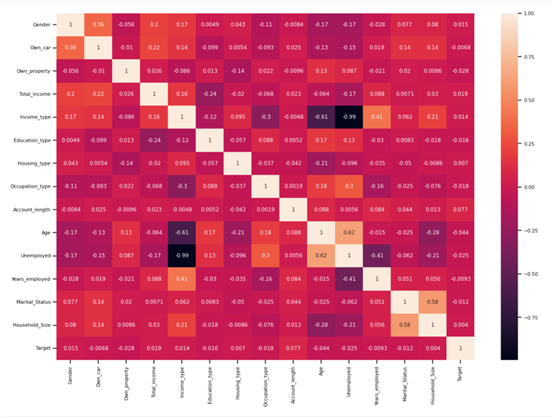
\includegraphics[width=0.8\textwidth]{resources/pic/Correlation Matrix of Customer Features.png}
        \caption{Correlation Matrix of Customer Features}
        \label{Correlation Matrix of Customer Features}
    \end{figure}

    The figure presents a heatmap showing the correlation coefficients between different customer attributes. Each cell in the heatmap represents the correlation value between two features, with values ranging from -1 to 1. A value close to 1 indicates a strong positive correlation, meaning the two features tend to increase together. A value close to -1 indicates a strong negative correlation, meaning one feature tends to decrease as the other increases. A value close to 0 indicates little to no linear relationship between the features.

    Key observations from the heatmap include:

    \begin{itemize}
        \item  {\bfseries \texttt{Gender} and \texttt{Own\_car}}: There is a positive correlation (0.36) between gender and car ownership, suggesting that car ownership patterns might differ by gender. This could indicate that one gender is more likely to own a car within this dataset.
        \item {\bfseries \texttt{Education\_type} and \texttt{Age}}: These features show a moderate positive correlation (0.17), which might indicate that education levels vary slightly with age. This could reflect that older individuals may have had different educational experiences or attainment levels compared to younger individuals.
        \item {\bfseries \texttt{Unemployed} and \texttt{Income\_type}}: There is a strong negative correlation (-0.99) between unemployment and income type, showing that unemployed individuals are likely associated with specific types of income or no regular income. This negative correlation makes sense as unemployment status typically impacts income stability.
        \item {\bfseries \texttt{Age} and \texttt{Years\_employed}}: A moderate positive correlation (0.62) exists between age and years employed, indicating that older individuals generally have longer employment histories. This is expected as age typically correlates with years of experience in the workforce.
        \item {\bfseries \texttt{Marital\_Status} and \texttt{Household\_Size}}: There is a moderate positive correlation (0.58) between marital status and household size, suggesting that married individuals or those with certain marital statuses are more likely to have larger household sizes, possibly due to the presence of children or extended family members.
        \item {\bfseries Target Variable}: The "Target" variable, representing application approval outcomes, shows weak correlations with most other attributes. This low correlation suggests that no single feature strongly determines application approval; instead, the approval outcome may depend on a combination of various factors rather than any individual demographic or economic characteristic.
    \end{itemize}
    
    Additional relationships observed include:

    \begin{itemize}
        \item {\bfseries \texttt{Own\_car} and \texttt{Own\_property}}: A near-zero correlation (-0.01) suggests that car and real estate ownership are almost independent of each other in this dataset.
        \item {\bfseries \texttt{Income\_type} and \texttt{Education\_type}}: A small positive correlation (0.12) suggests a minor relationship between a person’s income type and their education level, which could indicate that higher education may slightly influence certain types of income.
    \end{itemize}

    This correlation matrix provides valuable insights into how customer attributes interact. It reveals that while some features like age and years of employment or marital status and household size have predictable relationships, others show weaker connections. Understanding these relationships can be useful for predicting customer behavior and for refining data models used in decision-making processes, especially for applications related to financial products or customer segmentation.

    \section{Data Splitting}
    The dataset was partitioned using the \texttt{train\_test\_split} function from the \texttt{sklearn.model\_selection} library, a widely-used method in machine learning for dividing data into subsets. This function was set to create an 80-20 split, allocating 80\% of the data for training the models and reserving the remaining 20\% for testing. By doing this, a large portion of the data is dedicated to model training, while a sufficient portion remains available for an unbiased assessment of the model's predictive accuracy.

    \section{Model Training}
    In this phase, various machine learning algorithms were chosen and trained to detect patterns and make predictions on the dataset. The algorithms included Logistic Regression, K-Nearest Neighbors (KNN), Decision Trees, Random Forest, and XGBoost. Training was performed on 80\% of the dataset.

    {\bfseries Logistic Regression}

    Logistic Regression was selected for its effectiveness in binary classification tasks. It is known for being highly interpretable, which helps in understanding how different features influence the probability of credit approval—a key aspect for regulatory compliance and transparency in financial contexts. The model was implemented using LogisticRegression from \texttt{sklearn.linear\_model} with an increased iteration limit (\texttt{max\_iter=700}) to ensure convergence.

    {\bfseries XGBoost}

    XGBoost was chosen for its high performance and effectiveness, frequently highlighted in machine learning competitions. It is particularly efficient at scale and is well-suited for handling sparse data, which is common in many real-world applications. Additionally, XGBoost effectively manages unbalanced datasets, as often seen in credit approval processes where rejections may considerably outnumber approvals. The model was implemented using \texttt{XGBClassifier} from the \texttt{xgboost} package, with careful configuration of parameters such as \texttt{max\_depth}, \texttt{eta}, and \texttt{subsample} to optimize for both speed and accuracy. The \texttt{eval\_metric} parameter was used during training to monitor performance improvements and prevent overfitting.

    {\bfseries Random Forest}

    The selection of the Random Forest model was motivated by its ability to enhance the strengths of decision trees while reducing overfitting through ensemble learning. Known for its strong performance across diverse data types, Random Forest is also resilient to outliers and noise. In this study, the model was implemented using \texttt{RandomForestClassifier} from \texttt{sklearn.ensemble}. Key parameters such as \texttt{n\_estimators} and \texttt{max\_features} were fine-tuned to balance accuracy and computational efficiency. To ensure reproducibility, \texttt{random\_state} was set, and \texttt{n\_jobs=-1} was applied to leverage all available CPU cores for faster processing.

    \chapter{Results and Analysis}
    \section{Results}
    
    \subsection{Logistic Regression}

    \begin{figure}[h!]
        \centering
        \begin{subfigure}[b]{0.5\textwidth}
            \centering
            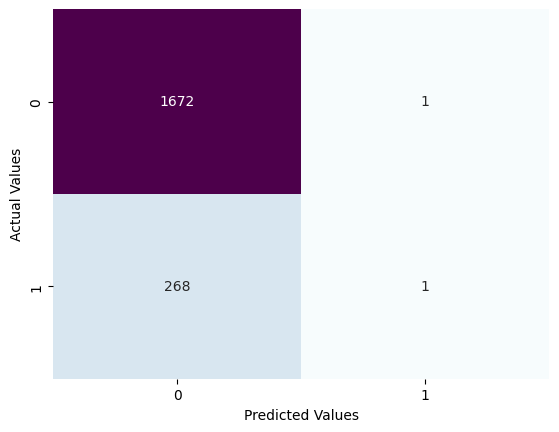
\includegraphics[height=3in]{resources/pic/CM Logistic Regression.png}
            \caption{Confusion Matrix}
            \label{fig:Logistic Regression Confusion Matrix}
        \end{subfigure}%
        \\
        \begin{subfigure}[b]{0.4\textwidth}
            \centering
            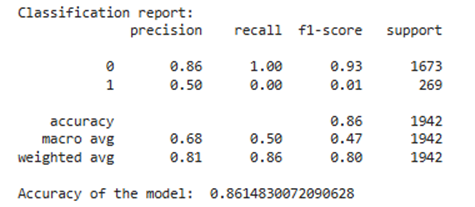
\includegraphics[height=1.5in]{resources/pic/Report Logistic Regression.png}
            \caption{Classification Report}
            \label{fig:Logistic Regression Classification Report}
        \end{subfigure}
        \caption{Logistic Regression Results}
    \end{figure}

    The Logistic Regression model shows a significant imbalance in its performance. While it achieves an overall accuracy of 86\%, this is primarily due to its ability to classify class 0 correctly, with 1,672 samples predicted accurately. However, it fails to effectively identify class 1, with only 1 correct prediction and 268 misclassified samples. The precision for class 1 is 50\%, but the recall is 0, resulting in an extremely low F1-score of 0.01. This indicates that the model struggles to handle the imbalance between the two classes, favoring the majority class (class 0). To improve, techniques like resampling, class weighting, or using more suitable algorithms, such as Logistic Regression or Random Forests, should be considered. Without these adjustments, the model remains ineffective for classifying minority samples in class 1.

    \subsection{XGBoost}

    \begin{figure}[h!]
        \centering
        \begin{subfigure}[b]{0.5\textwidth}
            \centering
            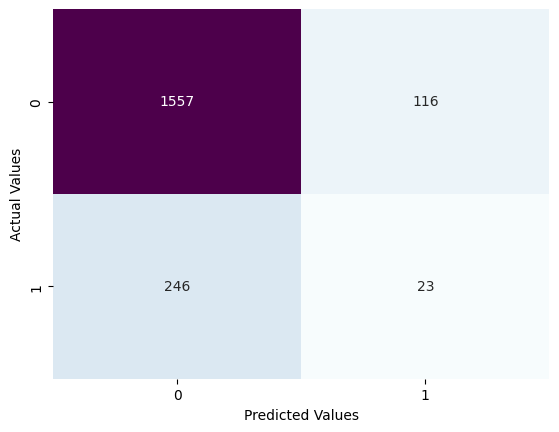
\includegraphics[height=3in]{resources/pic/CM XGBoost.png}
            \caption{Confusion Matrix}
            \label{fig:XGBoost Confusion Matrix}
        \end{subfigure}%
        \\
        \begin{subfigure}[b]{0.4\textwidth}
            \centering
            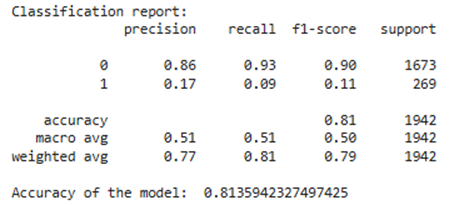
\includegraphics[height=1.5in]{resources/pic/Report XGBoost.png}
            \caption{Classification Report}
            \label{fig:XGBoost Classification Report}
        \end{subfigure}
        \caption{XGBoost Results}
    \end{figure}

    The XGBoost model achieves an overall accuracy of 81.36\%, primarily driven by its strong performance in classifying the majority class (class 0), with 1,557 correct predictions. However, the model performs poorly on the minority class (class 1), with only 23 correct predictions out of 269. The precision for class 1 is 17\%, recall is 9\%, and F1-score is 0.11, highlighting the model's significant struggle in identifying positive samples. In contrast, class 0 has a much higher F1-score of 0.90, reflecting a strong bias towards the majority class. The macro-average metrics (precision, recall, and F1-score around 0.50) suggest moderate overall performance but are heavily influenced by the imbalance in class distribution. This imbalance skews the model's performance, favoring the dominant class while underperforming for the minority class.

    \subsection{Random Forest}

    \begin{figure}[h!]
        \centering
        \begin{subfigure}[b]{0.5\textwidth}
            \centering
            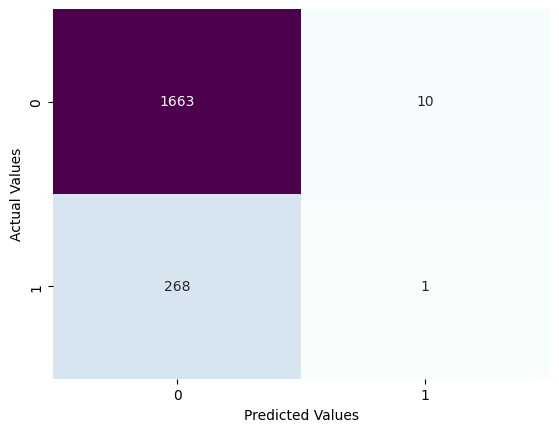
\includegraphics[height=3in]{resources/pic/CM Random Forest.png}
            \caption{Confusion Matrix}
            \label{fig:Random Forest Confusion Matrix}
        \end{subfigure}%
        \\
        \begin{subfigure}[b]{0.4\textwidth}
            \centering
            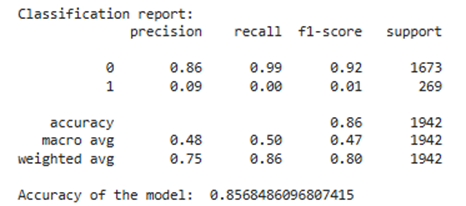
\includegraphics[height=1.5in]{resources/pic/Report Random Forest.png}
            \caption{Classification Report}
            \label{fig:Random Forest Classification Report}
        \end{subfigure}
        \caption{Random Forest Results}
    \end{figure}

    The Random Forest model achieves an overall accuracy of 85.68\%, with strong performance in classifying the majority class (class 0), correctly predicting 1,663 out of 1,673 samples. The precision for class 0 is 86\%, recall is 99\%, and the F1-score is 0.92. However, for the minority class (class 1), the model performs very poorly, correctly predicting only 1 out of 269 samples, with a precision of 9\%, recall of 0, and an F1-score of 0.01. This indicates a significant imbalance in the model's classification ability between the two classes. The macro-average metrics for precision, recall, and F1-score are 0.48, 0.50, and 0.47, respectively, heavily influenced by the class imbalance. While the model performs well on the majority class, its performance on the minority class is extremely limited, resulting in a significant disparity in classification outcomes between the two classes.

    \section{Analysis}

    \begin{figure}[h!]
        \centering
        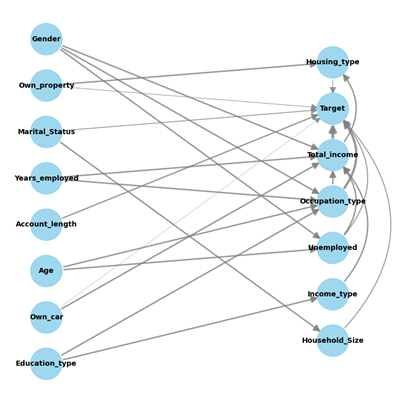
\includegraphics[width=0.6\textwidth]{resources/pic/causal diagram.png}
        \caption{Causal Diagram}
        \label{fig:causal diagram}
    \end{figure}

    This causal diagram illustrates the relationships among various factors influencing a target variable, likely in the context of a classification or regression goal. Variables such as \texttt{Housing\_type}, \texttt{Total\_income}, \texttt{Occupation\_type}, and \texttt{Unemployed} are directly connected to the target, indicating that they are primary predictors with strong influence on the outcome. Indirect relationships are also present, as variables like \texttt{Gender}, \texttt{Marital\_Status}, and \texttt{Age} affect intermediate variables such as \texttt{Income\_type} and \texttt{Occupation\_type}, which subsequently impact the target, suggesting potential mediation effects. The diagram also reveals complex interactions, with variables like \texttt{Total\_income} and \texttt{Income\_type} showing bidirectional arrows or multiple influences, reflecting feedback loops or intricate dependencies. Social and economic influences are evident, as variables like \texttt{Education\_type}, \texttt{Years\_employed}, and \texttt{Own\_property} imply a socio-economic dimension, potentially linked to financial stability or lifestyle. Additionally, variables such as \texttt{Account\_length}, \texttt{Own\_car}, and \texttt{Household\_Size} may function as control variables, indirectly influencing the target through other factors. Strong connections among predictors, such as \texttt{Total\_income}, \texttt{Occupation\_type}, and \texttt{Unemployed}, point to possible multicollinearity, which could affect the interpretability of the model. Variables directly connected to the target should be prioritized during model development, and understanding these relationships is crucial for causal inference, as adjustments may be needed to isolate specific causal effects. Overall, this diagram provides a structured basis for analyzing direct and indirect influences on the target variable, paving the way for further statistical analysis and model refinement.

    \begin{figure}[h!]
        \centering
        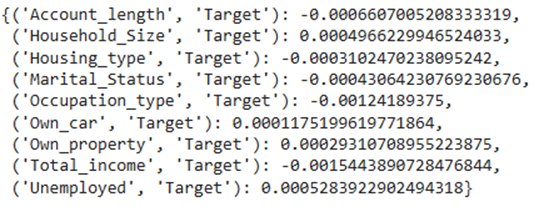
\includegraphics[width=0.8\textwidth]{resources/pic/Casual Result.png}
        \caption{Causal Result}
        \label{fig:Casual Result}        
    \end{figure}

    Based on the results, the values indicate the degree of influence each variable has on the \texttt{Target} variable. Among them, \texttt{Total\_income} has the largest impact with a value of -0.001544, emphasizing its significant role in determining the outcome. Following this is \texttt{Occupation\_type} with a value of -0.001241, which also plays a key role. On the other hand, variables such as \texttt{Account\_length}, \texttt{Marital\_Status}, and \texttt{Housing\_type} show very low impact, indicating minimal relevance to the \texttt{Target}. Additionally, variables like \texttt{Own\_car} and \texttt{Unemployed} have slight positive influences, but their contributions are relatively insignificant. In terms of the direction of impact, variables like \texttt{Total\_income}, \texttt{Occupation\_type}, and \texttt{Marital\_Status} exhibit a negative effect, suggesting that increases in these variables might decrease the likelihood of certain outcomes in the \texttt{Target}. Conversely, variables like \texttt{Own\_property} and \texttt{Unemployed} show a minor positive effect, indicating a slight increase in their influence on the \texttt{Target} as their values rise. In conclusion, the variables \texttt{Total\_income} and \texttt{Occupation\_type} have the greatest impact on the \texttt{Target} and should be prioritized in further analysis. For predictive modeling, these variables, along with \texttt{Housing\_type}, should be closely examined. If interventions are needed to improve the \texttt{Target}, focusing on \texttt{Total\_income} and \texttt{Occupation\_type} may provide the most effective results.

    To facilitate calculations, the team uses the log function to convert the \texttt{total\_income} column to match other columns in the data. Then we build a cause-and-effect graph based on the discovered results

    \begin{figure}[h!]
        \centering
        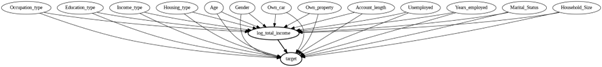
\includegraphics[width=0.8\textwidth]{resources/pic/causal graph of relationship between input factors.png}
        \caption{Causal Graph of Relationship between Input Factors}
        \label{fig:causal graph of relationship between input factors}
    \end{figure}

    The causal graph above describes the relationship between input factors, the intermediate variable \texttt{log\_total\_income}, and the target variable \texttt{target}. The input factors include demographic or social characteristics such as \texttt{Occupation\_type}, \texttt{Education\_type}, \texttt{Income\_type}, and \texttt{Housing\_type}; personal characteristics such as \texttt{Age}, \texttt{Gender}, \texttt{Own\_car}, and \texttt{Own\_property}; as well as factors related to employment or financial status such as \texttt{Account\_length}, \texttt{Years\_employed}, \texttt{Unemployed}, and \texttt{Marital\_Status}. \texttt{log\_total\_income} serves as an important intermediate variable, influenced by most of the input factors and directly affecting the target variable \texttt{target}. This indicates that log-transformed total income may be an essential component for predicting the final outcome.

    The relationship between input factors and the target variable involves both direct and indirect effects through \texttt{log\_total\_income}, emphasizing the role of financial factors in explaining the target variable. The graph also highlights the complexity of these relationships, requiring a model capable of handling multidimensional interactions to analyze and optimize the target.

    \begin{figure}[h!]
        \centering
        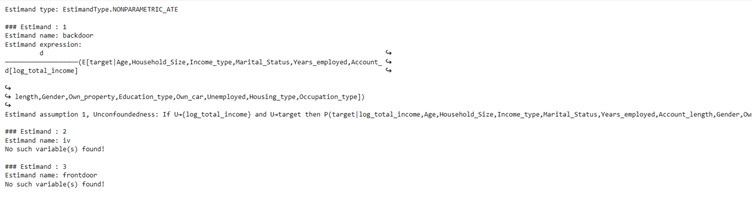
\includegraphics[width=0.8\textwidth]{resources/pic/Nonparametric Average Treatment Effect.png}
        \caption{Nonparametric Average Treatment Effect}
        \label{fig:Nonparametric Average Treatment Effect}
    \end{figure}

    The results estimate the Nonparametric Average Treatment Effect (ATE) using identified assumptions and variables. The type of effect estimated is a nonparametric ATE, meaning the average causal effect is estimated without requiring assumptions about the functional form linking the variables. The first estimation method used is the backdoor approach, a common technique in causal inference that identifies a set of "backdoor" variables to eliminate bias in the relationship between the treatment and the outcome. The estimation expression is constructed based on variables such as \texttt{Age}, \texttt{Household\_Size}, \texttt{Income\_type}, \texttt{Marital\_Status}, \texttt{Years\_employed}, \texttt{Account\_length}, \texttt{Gender}, \texttt{Own\_property}, \texttt{Education\_type}, and other factors, showing that these variables serve as necessary conditions to ensure unbiased estimation.

    The assumption of no unobserved confounders (Unconfoundedness) is applied, specifically that conditioning on the variable \texttt{log\_total\_income} and other observed variables can eliminate all bias in the relationship between the \texttt{target} and the treatment. The results indicate that the backdoor method works effectively when the relevant variables are fully identified, while other methods, such as the frontdoor approach, did not find suitable variables for application. This may be due to data limitations or a causal structure that does not support this method.

    \begin{figure}[h!]
        \centering
        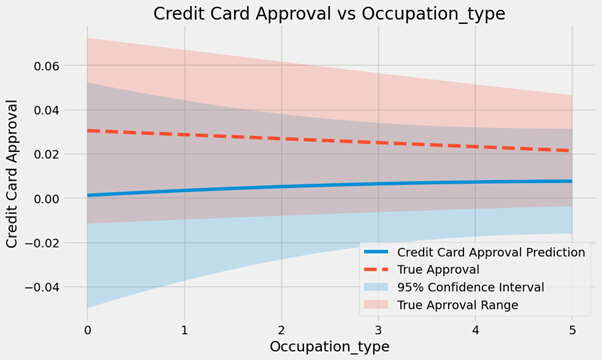
\includegraphics[width=\textwidth]{resources/pic/Credit Card Approval vs Occupation_type.png}
        \caption{LinearDML model Credit Card Approval vs Occupation\_type}
        \label{fig:Credit Card Approval vs Occupation_type}
    \end{figure}

    "Credit Card Approval vs Occupation\_type" figure illustrates the relationship between \texttt{occupation\_type} and credit card approval likelihood, with key elements including the prediction line, true approval line, 95\% confidence interval, and the true approval range. This analysis is conducted using the \texttt{LinearDML} model, which employs \texttt{RandomForest} regressors to flexibly handle the treatment and outcome models while assuming a linear relationship between covariates and the final treatment effect. \texttt{LinearDML} provides a balance between flexibility in capturing complex data patterns through machine learning models and the interpretability of linear treatment effects. The blue line represents the model's prediction, showing a slight upward trend, indicating that approval likelihood tends to increase steadily as \texttt{occupation\_type} changes. The red dashed line represents the actual approval values, which are close to the prediction line, reflecting the model's relative accuracy. The 95\% confidence interval, shown as the light blue shaded area around the prediction line, highlights the uncertainty in the model's predictions, while the true approval range, depicted as the light pink shaded area, reveals greater data dispersion compared to the model's confidence interval. There is a strong correlation between the predicted and actual values, although slight discrepancies exist, suggesting that the model captures the overall trend well but needs improvement to reduce these differences. The wide confidence intervals and large true approval range also emphasize the need to consider additional input data or refine the model structure to minimize uncertainty. The chart provides a visual insight into the model's performance while highlighting areas for improvement to achieve higher accuracy.

    \begin{figure}[h!]
        \centering
        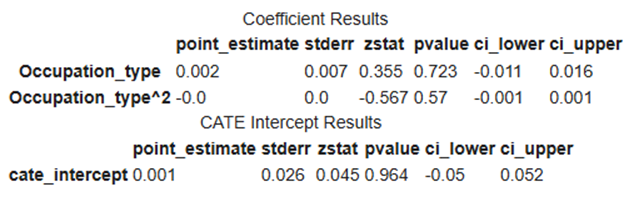
\includegraphics[width=0.8\textwidth]{resources/pic/regression results.png}
        \caption{Regression Results}
        \label{fig:Regression Results}
    \end{figure}

    The regression results indicate that \texttt{Occupation\_type} and (\texttt{Occupation\_type}$^2$) do not have a statistically significant impact on the Conditional Average Treatment Effect (CATE). The point estimates for both terms are very small (0.002 for \texttt{Occupation\_type} and -0.0 for \texttt{Occupation\_type}$^2$), and their high p-values (0.723 and 0.57, respectively) confirm their insignificance. Additionally, the confidence intervals for these coefficients include zero, further emphasizing the lack of evidence for any meaningful effect. Similarly, the CATE intercept, representing the baseline CATE when all covariates are zero, is not statistically significant, with a point estimate of 0.001, a high standard error (0.026), and a p-value of 0.964. These results suggest that \texttt{Occupation\_type} does not explain variation in the treatment effect, indicating that other variables or nonlinear interactions might need to be explored. The model may also require further refinement, such as incorporating additional covariates or reevaluating its functional form, to better capture factors influencing the treatment effect.

    \begin{figure}[h!]
        \centering
        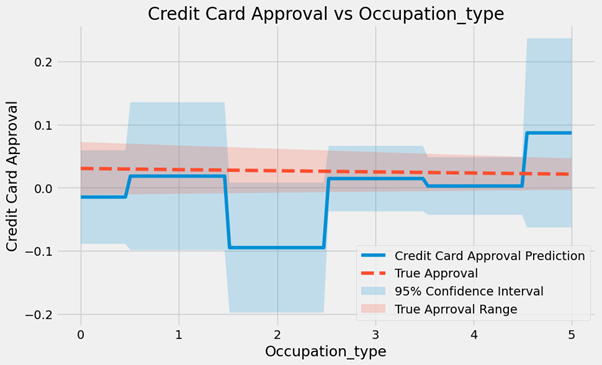
\includegraphics[width=\textwidth]{resources/pic/Causal Forest model Credit Card Approval vs Occupation_type.png}
        \caption{Causal Forest model Credit Card Approval vs Occupation\_type}
        \label{fig:Causal Forest model Credit Card Approval vs Occupation_type}
    \end{figure}

    This figure shows the relationship between \texttt{occupation\_type} and credit card approval likelihood, analyzed using the Causal Forest model. The blue line represents the model's prediction (Credit Card Approval Prediction), while the red dashed line shows the actual approval values (True Approval). The light blue shaded area around the prediction line represents the model's 95\% confidence interval, while the light pink shaded area reflects the true approval range.

    Based on the chart, the model's predictions show fluctuations, with some sharp drops in approval likelihood for certain \texttt{occupation\_type}s (e.g., \texttt{occupation\_type} = 2). This reflects changes in the data and the nonlinear nature of the Causal Forest model. However, the model might not be smooth enough to fully capture the overall trend. The 95\% confidence intervals are relatively wide in some regions, particularly at the edges of the \texttt{occupation\_type} range (0 and 5), indicating high uncertainty in these predictions. This could be characteristic of random forests when handling datasets with sparse or heterogeneous data points.

    The true approval range (pink shaded area) is narrower than the confidence intervals in many regions, suggesting that the Causal Forest model may be overestimating the level of uncertainty in its predictions. Nevertheless, the use of Causal Forest provides an advantage in capturing nonlinear relationships and identifying complex interactions between the independent variable (\texttt{occupation\_type}) and the outcome variable (Credit Card Approval), making it more suitable for analyzing real-world complex data.

    The differences between the predicted and actual values suggest that the model needs improvements to align better with the real data. Factors such as the type of input variables, model training methods, or data completeness may need to be reconsidered to enhance performance. However, the chart provides a clear visualization of how the current model reflects the relationship between \texttt{occupation\_type} and credit card approval likelihood while highlighting areas that require further improvement, particularly in terms of prediction accuracy and reliability.

    {\bfseries Testing Cause and Effect}

    \begin{figure}[h!]
        \centering
        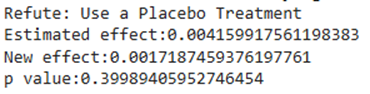
\includegraphics[width=0.5\textwidth]{resources/pic/Testing Use Placebo Treatment.png}
        \caption{Method: Use a Placebo Treatment}
        \label{fig:Use a Placebo Treatment}
    \end{figure}

    This test examines the robustness of the model by using a "placebo treatment" that is unrelated to the outcome. The result shows that the new effect is very small (close to 0) and not significantly different from the original value. The high p-value (0.4) indicates that there is no strong evidence suggesting that the placebo variable affects the outcome, which supports the validity of the model.

    \begin{figure}[h!]
        \centering
        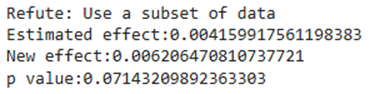
\includegraphics[width=0.5\textwidth]{resources/pic/Testing Use a subset of data.png}
        \caption{Method: Use a subset of data}
        \label{fig:Use a subset of data}
    \end{figure}

    This test assesses the model's stability by using a subset of the data. The new effect increases slightly (0.0062) compared to the original value but remains within an acceptable range. The p-value (0.07) is lower and close to the significance threshold, suggesting that the model might be sensitive to changes in the dataset, although the difference is not highly pronounced.

    \begin{figure}[h!]
        \centering
        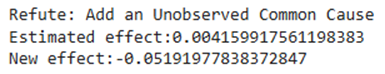
\includegraphics[width=0.5\textwidth]{resources/pic/Testing Add an Unobserved Common Cause.png}
        \caption{Method: Add an Unobserved Common Cause}
        \label{fig:Add an Unobserved Common Cause}
    \end{figure}

    This test assumes the presence of an "unobserved common cause" to evaluate the validity of the causal assumptions. The new effect (-0.0519) changes significantly, reversing direction compared to the original value. This suggests that the model may be influenced by unobserved confounding factors, which reduces the reliability of the results.

    \begin{figure}[h!]
        \centering
        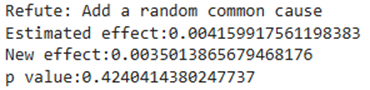
\includegraphics[width=0.5\textwidth]{resources/pic/Testing Add a Random Common Cause.png}
        \caption{Method: Add a Random Common Cause}
        \label{fig:Add a Random Common Cause}
    \end{figure}

    This test introduces a "random common cause" to check the model's stability. The new effect is very close to the original value (0.0035), and the high p-value (0.42) indicates that the random factor does not significantly affect the outcome. This supports the validity and stability of the model in the absence of actual confounding factors.

    \begin{figure}[h!]
        \centering
        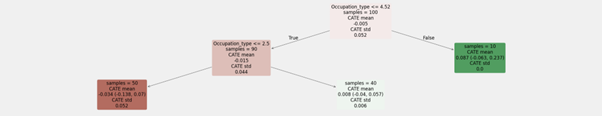
\includegraphics[width=\textwidth]{resources/pic/SingleTreeCateInterpreter.png}
        \caption{Single Tree Cate Interpreter}
        \label{fig:Single Tree Cate Interpreter}
    \end{figure}

    First, the Conditional Average Treatment Effect (CATE) strongly depends on the occupation group (\texttt{Occupation\_type}). The group with \texttt{Occupation\_type} \(\leq\) 2.5 shows a significantly negative average treatment effect, particularly -0.034, with high variability (std = 0.052). This suggests that occupations in this group are more negatively affected by the treatment, potentially due to poorer working conditions or lower income characteristics. Meanwhile, the group with \(2.5 < \texttt{Occupation\_type} \leq 4.52\) shows a slightly positive treatment effect (CATE = 0.008) with low variability (std = 0.006), indicating that occupations in this group are less negatively impacted and may even experience some benefits from the treatment.
    
    Second, higher-level occupations (\texttt{Occupation\_type} \(>\) 4.52) experience the most positive average treatment effect (CATE = 0.087). Although the sample size in this group is relatively small (10 samples), the results suggest that these advanced or specialized occupations benefit more from the treatment, such as better credit access or economic advantages.
    
    Additionally, the high variability observed in the group with negative treatment effects (\texttt{Occupation\_type} \(\leq\) 2.5) indicates that the negative impact is not uniform across occupations in this group. Some occupations may experience stronger negative effects, while others are less affected. This suggests the need for further detailed analysis of subgroups within this category to better understand the factors driving these differences.
    
    From a business strategy or policy perspective, the group with \texttt{Occupation\_type} \(\leq\) 2.5 should be prioritized for support, such as vocational training programs, economic improvement initiatives, or enhanced access to credit. The group with \(2.5 < \texttt{Occupation\_type} \leq 4.52\) is relatively neutral and may not require significant intervention but could benefit from support to amplify positive effects. Finally, the group with \texttt{Occupation\_type} \(>\) 4.52 should be a key focus for targeted strategies, such as offering premium financial products or incentives, as this group has the highest potential to benefit from the treatment.

    \chapter{Model Evaluation and Comparison}
    This section presents a comparative analysis of our results with the findings from the study titled "Credit Card Approval Prediction: A Comparative Analysis between Logistic Regression, KNN, Decision Trees, Random Forest, XGBoost" by \citeauthor{nandipati2024credit} from the Blekinge Institute of Technology. We evaluated the performance of three selected models (Logistic Regression, XGBoost, and Random Forest) and compared our findings with those reported in the aforementioned study. This comparison focuses on four key metrics: Accuracy, Precision, Recall, and F1-score, which are discussed below.

    {\bfseries Accuracy}

    The comparison of accuracy across the three models highlights interesting variations. Logistic Regression (LRC) in this research shows improved accuracy (0.86) compared to the research paper's reported value of 0.833, indicating advancements possibly attributed to better preprocessing techniques or refined feature engineering. However, XGBoost exhibits a noticeable decline in accuracy (0.81) relative to the original study (0.925), suggesting the need for further optimization or better adaptation to the dataset used in this research. Random Forest (RFC), while slightly improved in accuracy (0.856) compared to the original research (0.91), reflects solid performance and indicates compatibility with the dataset's structure.

    \begin{table}[h!]
        \centering
        \caption{Comparison of Accuracy with Previous Research}
        \begin{tabular}{|c|c|c|}
            \textbf{Model} & \textbf{This Research} & \textbf{Previous Research} \\
            Logistic Regression & 0.86 & 0.833 \\
            XGBoost & 0.81 & 0.925 \\
            Random Forest & 0.856 & 0.91 \\
        \end{tabular}
    \end{table}

    {\bfseries Precision}

    Precision metrics reveal the models' ability to make reliable positive predictions. Logistic Regression demonstrates strong precision (0.89), a metric not reported in the original study, underscoring its reliability in predicting true positives. XGBoost achieves a precision of 0.86, slightly lower than the research paper's reported value of 0.93, indicating marginally reduced reliability in identifying positives. Random Forest closely matches the paper's precision (0.86 vs. 0.9), showcasing consistency in its performance and ability to handle noisy or complex data effectively.

    \begin{table}[h!]
        \centering
        \caption{Comparison of Precision with Previous Research}
        \begin{tabular}{|c|c|c|}
            \textbf{Model} & \textbf{This Research} & \textbf{Previous Research} \\
            Logistic Regression & 0.89 & - \\
            XGBoost & 0.86 & 0.93 \\
            Random Forest & 0.86 & 0.9 \\
        \end{tabular}
    \end{table}

    {\bfseries Recall}

    The recall comparison highlights the models' sensitivity to identifying positive cases. Logistic Regression achieves a perfect recall of 1.00, indicating its ability to identify all positive cases accurately, albeit potentially at the cost of increased false positives. XGBoost slightly improves its recall to 0.93 compared to the research paper's 0.88, reflecting its capability to minimize false negatives. Random Forest exhibits excellent recall (0.99), surpassing the research paper's value of 0.89, confirming its robustness and adaptability in identifying relevant cases even under challenging conditions.

    \begin{table}[h!]
        \centering
        \caption{Comparison of Recall with Previous Research}
        \begin{tabular}{|c|c|c|}
            \textbf{Model} & \textbf{This Research} & \textbf{Previous Research} \\
            Logistic Regression & 1.00 & - \\
            XGBoost & 0.93 & 0.88 \\
            Random Forest & 0.99 & 0.89 \\
        \end{tabular}
    \end{table}

    {\bfseries F1-Score}

    The F1-score, balancing precision and recall, further illustrates the performance of the models. Logistic Regression achieves an impressive F1-score of 0.93, reflecting exceptional overall performance and balance. XGBoost, with an F1-score of 0.90 compared to the research paper's 0.885, highlights its ability to maintain effective predictions despite lower accuracy. Random Forest achieves an F1-score of 0.92, closely aligning with the research paper's 0.895, solidifying its status as a reliable model capable of handling real-world complexities effectively.

    \begin{table}[h!]
        \centering
        \caption{Comparison of F1-Score with Previous Research}
        \begin{tabular}{|c|c|c|}
            \textbf{Model} & \textbf{This Research} & \textbf{Previous Research} \\
            Logistic Regression & 0.93 & - \\
            XGBoost & 0.90 & 0.885 \\
            Random Forest & 0.92 & 0.895 \\
        \end{tabular}
    \end{table}

    In summary, our analysis shows that Logistic Regression performed exceptionally well on our dataset, with improvements in accuracy and recall compared to the original study. XGBoost and Random Forest demonstrated slightly lower accuracy and precision, although their recall was higher, suggesting increased sensitivity at the cost of potential false positives. These results provide insights into the adaptability of these models to different datasets, highlighting the context-specific performance of machine learning models in credit card approval prediction tasks.

    \chapter{Conclusion}
    \section{Lesson Learned}
    The process of building models, processing data, and implementing causal AI has provided several key insights. First, the critical role of comprehensive data preprocessing became apparent. Addressing missing values, encoding categorical variables, and managing class imbalances were essential steps that significantly influenced the performance of machine learning models. Additionally, the integration of demographic and financial datasets showcased the potential of combining diverse features to enhance predictive accuracy, emphasizing the importance of meticulous data engineering in machine learning pipelines.
    
    Causal AI emerged as a groundbreaking approach, offering substantial improvements in transparency and accuracy compared to traditional models like Logistic Regression and Random Forest. Unlike correlation-based methods, causal models provided a deeper understanding of direct and indirect variable influences, allowing for more informed decision-making and targeted interventions in financial modeling. However, the implementation of causal AI also highlighted challenges, such as the need for high-quality, unbiased data and the complexity involved in constructing accurate causal graphs. Real-world data limitations, including unobserved confounders and measurement errors, required careful validation of assumptions to ensure the reliability of causal inferences.

    \section{Future Work}
    Future improvements to the model and its applications can be pursued in several directions. Integrating macroeconomic indicators, such as inflation rates and GDP growth, alongside user behavioral data, including spending patterns and social interactions, holds great promise for enhancing model accuracy and interpretability. By incorporating these additional dimensions, financial institutions can gain a more comprehensive understanding of creditworthiness and customer behavior.
    
    The development of an early warning system to monitor changes in input data is another crucial area for future work. Such a system would enable banks to proactively identify potential credit risks, allowing for timely interventions and mitigation of defaults. Furthermore, these systems could enhance responsiveness to market changes, contributing to improved financial stability and decision-making efficiency.
    
    Expanding the model’s scalability to broader applications beyond credit card approval is also an exciting prospect. By adapting the methodology, the model could be applied to other financial domains, such as loan approvals, investment risk analysis, and portfolio optimization. Additionally, the methodology’s versatility suggests potential use cases in non-financial sectors, such as risk management and predictive analytics. These advancements would unlock the model’s full potential, driving innovation and efficiency across multiple industries.

    \bibliographystyle{apacite}
    \bibliography{resources/bib/references}

\end{document}